\section*{Question 4:}
Exercise 6.9:

Give five examples of web page translation that you think is poor. Why do you think the translation failed?

\section*{Answer:}

The five web pages I have chosen are my home page, ODU's home page, Dr. Nelson's home page, Dr. Weigle's home page, and Mr. Kennedy's home page.

\begin{figure}[h]
\caption{Google Web Translation for hussam.us}
\centering
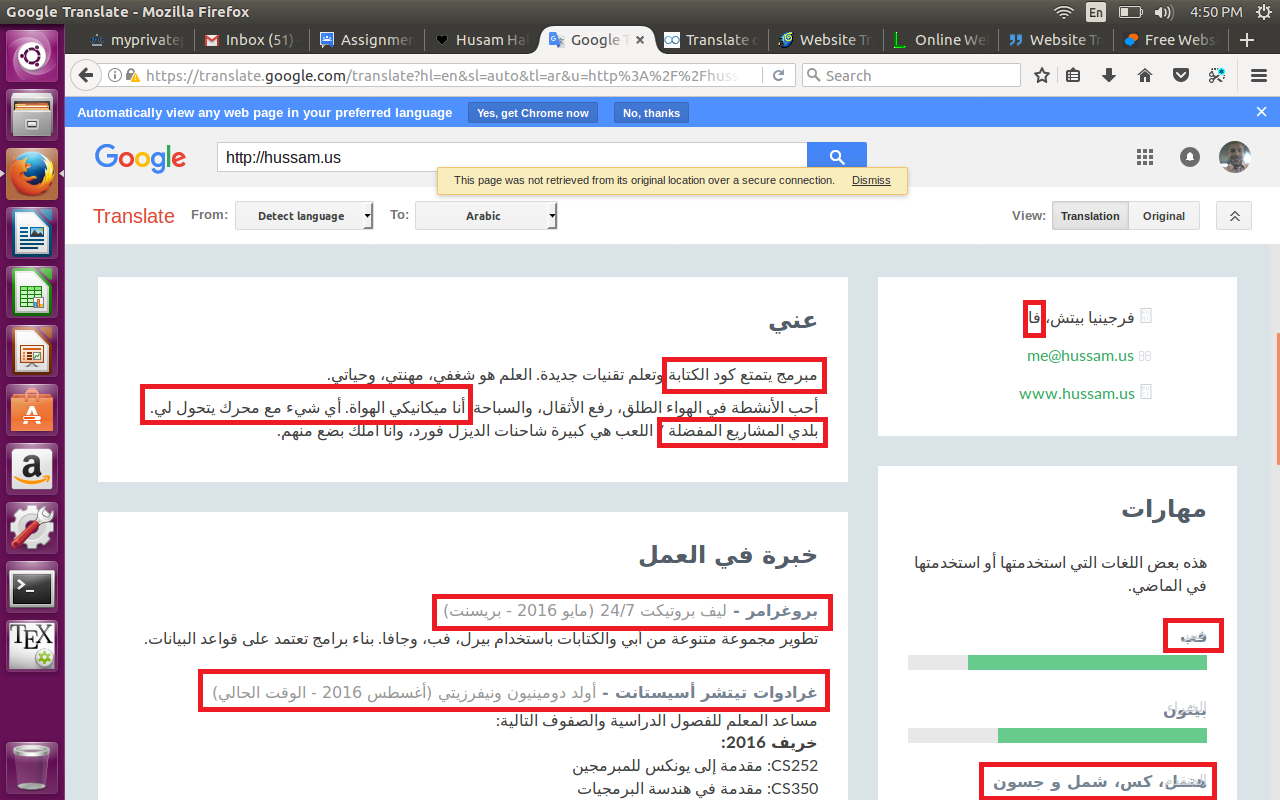
\includegraphics[scale=0.54]{Q4/1.png}
\end{figure}

\begin{figure}[h]
\caption{Google Web Translation for odu.edu}
\centering
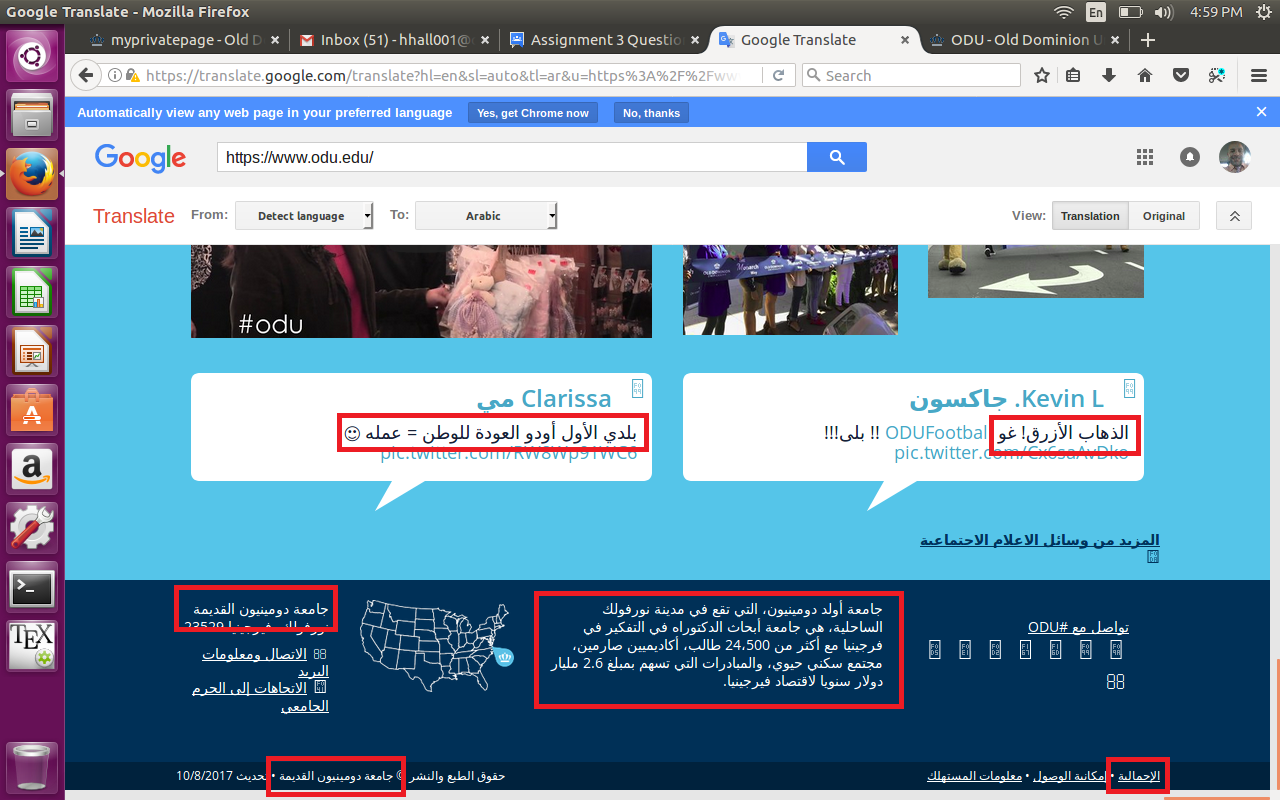
\includegraphics[scale=0.54]{Q4/2.png}
\end{figure}

\begin{figure}[h]
\caption{Google Web Translation for Dr. Nelson}
\centering
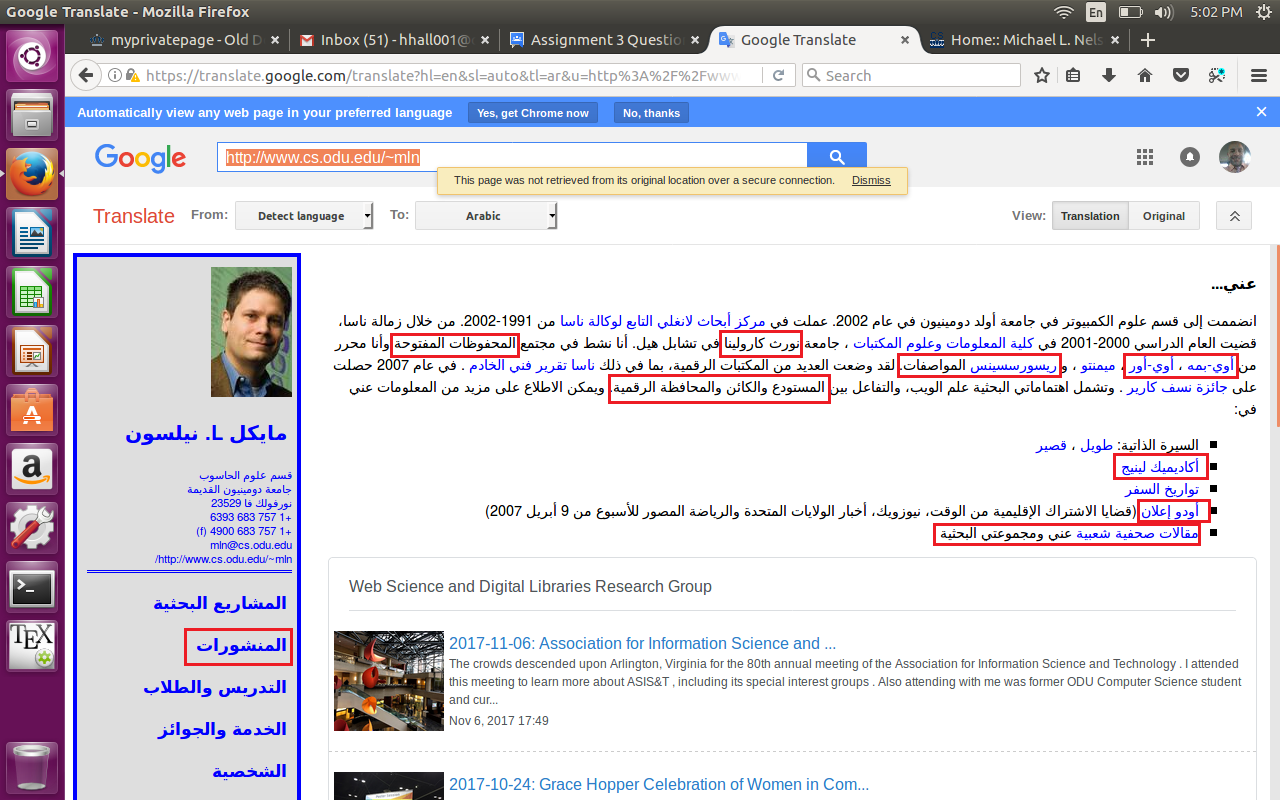
\includegraphics[scale=0.54]{Q4/3.png}
\end{figure}

\begin{figure}[h]
\caption{Google Web Translation for Dr. Weigle}
\centering
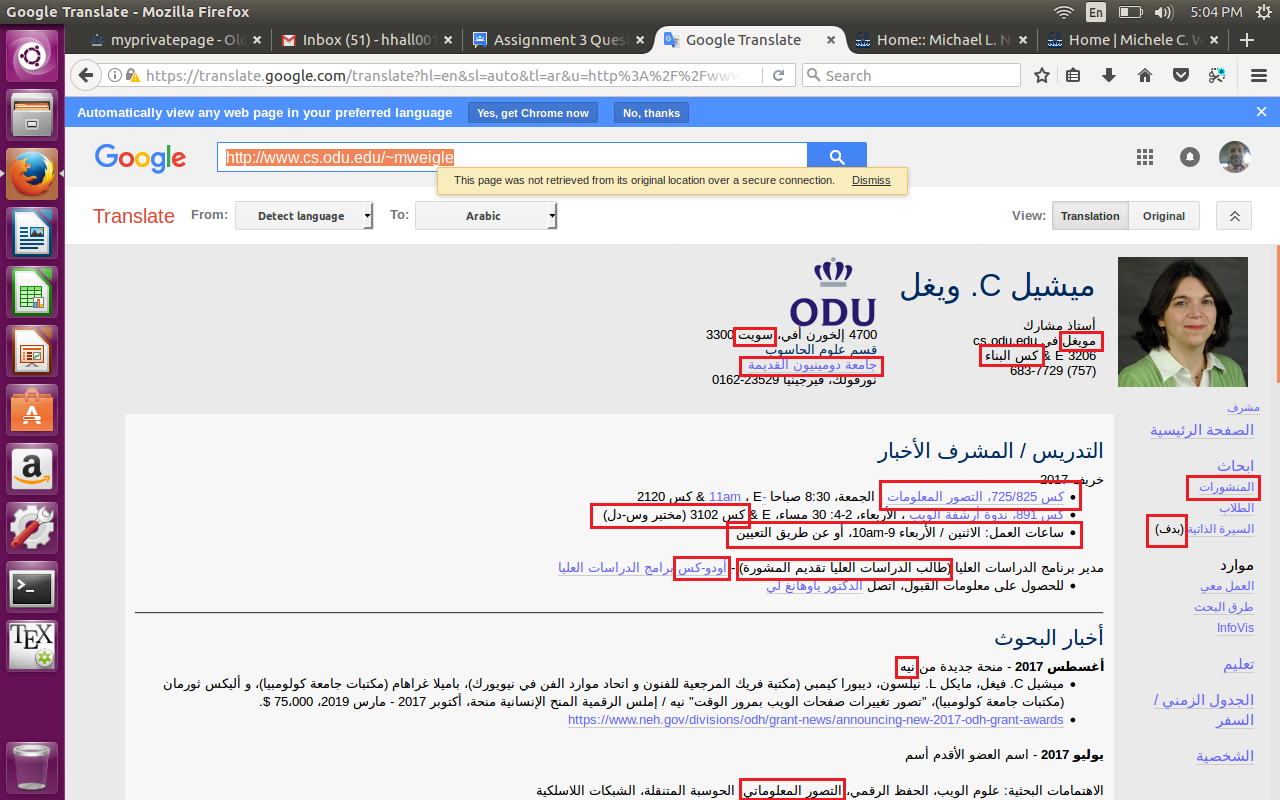
\includegraphics[scale=0.54]{Q4/4.png}
\end{figure}

\begin{figure}[h]
\caption{Google Web Translation for Mr. Kennedy}
\centering
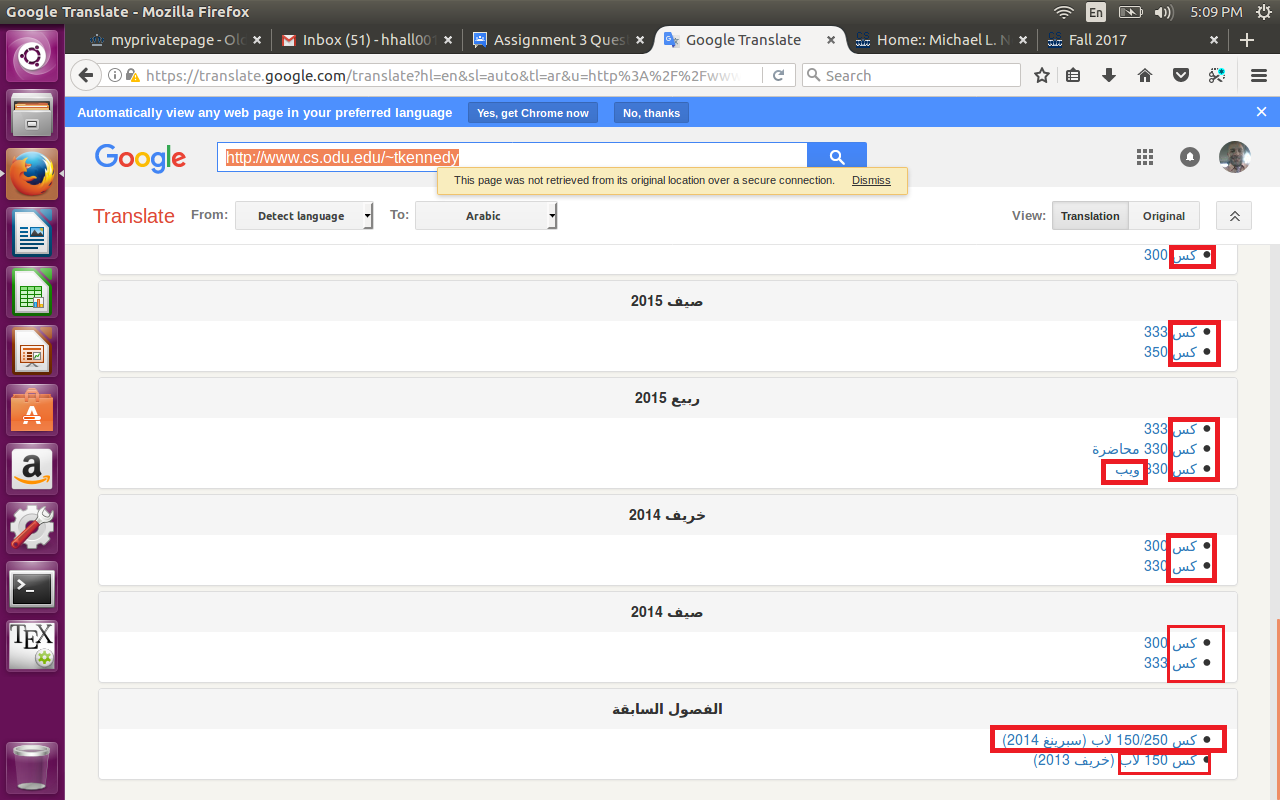
\includegraphics[scale=0.54]{Q4/5.png}
\end{figure}

I translated the pages using Google web pages translation service. The translation was from English to Arabic, my first language. I put red rectangles around the parts where the translation is poor. It is clear that the translation was poor and inconsistent on all five web pages, which I think is due to multiple reasons:

1. Acronyms unknown to the translator such as CS, ODU, VA, PHP, HTML, ...etc

2. Capitalization: Sometimes ``Spring'' is translated as spring, the season in Arabic, and sometimes it is transliterated as if ``Spring'' were a name of a person or business, ...etc. The translation was also inconsistent in this case. The same happened to the word ``Old'' in ``Old Dominion University''

3. Titles translation was always poor. The word ``Programmer'' was transliterated when it was in the title, but it was translated when it was in a paragraph.

4. Poor/informal English: One of the cases is the introduction on my home page. The first sentence is a fragment that ends with a period. I did not use first person, and made it sound like someone else is introducing me to the visitor. ``A programmer who enjoys writing code and learning new technologies.'' is a fragment ending with a period, which is probably what caused the translator to generate a very bad translation.

5. Words have multiple meanings depending on the context. The translator does not consider that when translating a web page. One example is the word ``Publications'' in Dr. Nelson's page. The Arabic translation makes it sound like it means published Facebook posts or tweets instead of published research papers. The reason is that the translator does not classify the page before translating it. If Google classified pages before translating them, the translation would be much better. The word ``Publications'' on a professor's home page could not mean published social media posts. It sure means something like published research papers, other scholarly documents, or at least articles.
